\documentclass[ngerman, aspectratio=169]{beamer}

%style
\mode<presentation>{
	\usetheme{Frankfurt}
}
%packages
\usepackage[utf8]{inputenc}
\usepackage[english]{babel}
\usepackage{graphicx}
\usepackage{array}

\newcolumntype{L}[1]{>{\raggedright\let\newline\\\arraybackslash\hspace{0pt}}m{#1}}
\usepackage{ragged2e}

\usepackage{bm} % bold math
\usepackage{amsfonts}
\usepackage{amssymb}
\usepackage{mathtools}
\usepackage{amsmath}
\usepackage{multirow} % multi row in tables
\usepackage{scrextend}

\usepackage{tikz}

\usepackage{algorithmic}

%\usepackage{algorithm} % http://ctan.org/pkg/algorithm
%\usepackage{algpseudocode} % http://ctan.org/pkg/algorithmicx

%\usepackage{algorithmicx}


%citations
\usepackage[style=verbose,backend=biber]{biblatex}
\addbibresource{references.bib}



\usefonttheme[onlymath]{serif}

%Beamer Template modifications
%\definecolor{mainColor}{HTML}{0065A3} % HSR blue
\definecolor{mainColor}{HTML}{D72864} % OST pink
\definecolor{invColor}{HTML}{28d79b} % OST pink
\definecolor{dgreen}{HTML}{38ad36} % Dark green

%\definecolor{mainColor}{HTML}{000000} % HSR blue
\setbeamercolor{palette primary}{bg=white,fg=mainColor}
\setbeamercolor{palette secondary}{bg=orange,fg=mainColor}
\setbeamercolor{palette tertiary}{bg=yellow,fg=red}
\setbeamercolor{palette quaternary}{bg=mainColor,fg=white} %bg = Top bar, fg = active top bar topic
\setbeamercolor{structure}{fg=black} % itemize, enumerate, etc (bullet points)
\setbeamercolor{section in toc}{fg=black} % TOC sections
\setbeamertemplate{section in toc}[sections numbered]
\setbeamertemplate{subsection in toc}{%
	\hspace{1.2em}{$\bullet$}~\inserttocsubsection\par}

\setbeamertemplate{itemize items}[circle]
\setbeamertemplate{description item}[circle]
\setbeamertemplate{title page}[default][colsep=-4bp,rounded=true]
\beamertemplatenavigationsymbolsempty

\setbeamercolor{footline}{fg=gray}
\setbeamertemplate{footline}{%
	\hfill\usebeamertemplate***{navigation symbols}
	\hspace{0.5cm}
	\insertframenumber{}\hspace{0.2cm}\vspace{0.2cm}
}

\usepackage{caption}
\captionsetup{labelformat=empty}

%Title Page
\title{Riemannsche Zeta Funktion}
\author{Raphael Unterer}
\institute{Mathematisches Seminar 2022: Spezielle Funktionen}

\newcommand*{\HL}{\textcolor{mainColor}}
\newcommand*{\RD}{\textcolor{red}}
\newcommand*{\BL}{\textcolor{blue}}
\newcommand*{\GN}{\textcolor{dgreen}}




\makeatletter
\newcount\my@repeat@count
\newcommand{\myrepeat}[2]{%
	\begingroup
	\my@repeat@count=\z@
	\@whilenum\my@repeat@count<#1\do{#2\advance\my@repeat@count\@ne}%
	\endgroup
}
\makeatother




\usetikzlibrary{automata,arrows,positioning,calc}


\begin{document}

	%Titelseite
	\begin{frame}
		\titlepage
	\end{frame}

	%Inhaltsverzeichnis
	\begin{frame}
		\frametitle{Inhalt}
		\tableofcontents
	\end{frame}

	\section{Motivation}

    \begin{frame}
        \frametitle{Summe aller Natürlichen Zahlen}
        \begin{equation*}
            \sum_{n=1}^{\infty} n
            =
            1 + 2 + 3 + \ldots + \infty
            =
            - \frac{1}{12}
        \end{equation*}
    \end{frame}
    \begin{frame}
        \frametitle{Summe aller Natürlichen Zahlen}
        \begin{center}
            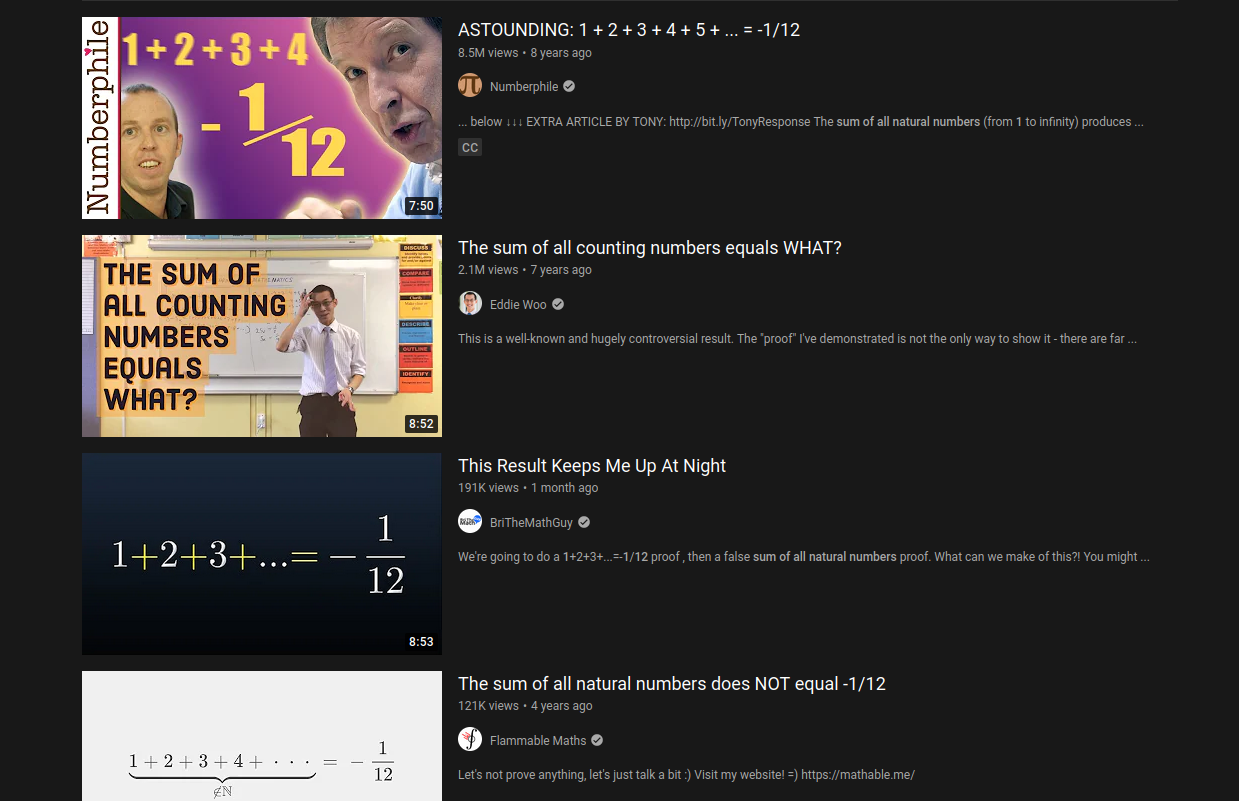
\includegraphics[width=0.7\textwidth]{youtube_screenshot.png}
        \end{center}
    \end{frame}
    \begin{frame}
        \frametitle{Riemannsche Zeta Funktion}
        \begin{equation*}
            \zeta(s)
            =
            \sum_{n=1}^{\infty}
            \frac{1}{n^s}
        \end{equation*}
        \pause
        \begin{equation*}
            \zeta(-1)
            =
            \sum_{n=1}^{\infty}
            \frac{1}{n^{-1}}
            =
            \sum_{n=1}^{\infty} n
        \end{equation*}
    \end{frame}
    \begin{frame}
        \frametitle{Originaler Definitionsbereich}
        Wir kennen die divergierende harmonische Reihe
        \begin{equation*}
            \zeta(1)
            =
            \sum_{n=1}^{\infty}
            \frac{1}{n}
            \rightarrow
            \infty,
        \end{equation*}
        und somit ist $\Re(s) > 1$.
    \end{frame}

    \section{Analytische Fortsetzung}
    \begin{frame}
        \frametitle{Plan für die Analytische Fortsetzung von $\zeta(s)$}
        \begin{center}
            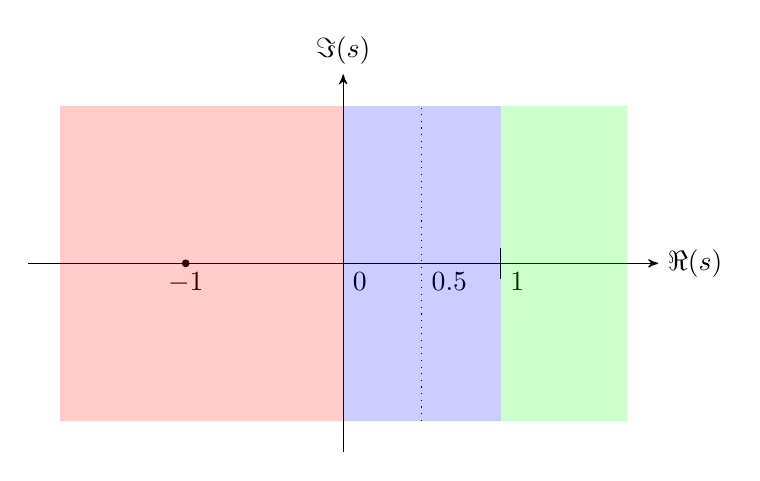
\begin{tikzpicture}[>=stealth', auto, node distance=0.9cm, scale=2,
    dot/.style={fill, circle, inner sep=0, minimum size=0.1cm}]

    \draw[->] (-2,0) -- (-1,0) node[dot]{} node[anchor=north]{$-1$} -- (0,0) node[anchor=north west]{$0$} -- (0.5,0) node[anchor=north west]{$0.5$}-- (1,0) node[anchor=north west]{$1$} -- (2,0) node[anchor=west]{$\Re(s)$};

    \draw[->] (0,-1.2) -- (0,1.2) node[anchor=south]{$\Im(s)$};
    \begin{scope}[yscale=0.1]
        \draw[] (1,-1) -- (1,1);
    \end{scope}
    \draw[dotted] (0.5,-1) -- (0.5,1);

    \begin{scope}[]
        \fill[opacity=0.2, red] (-1.8,1) rectangle (0, -1);
        \fill[opacity=0.2, blue] (0,1) rectangle (1, -1);
        \fill[opacity=0.2, green] (1,1) rectangle (1.8, -1);
    \end{scope}

\end{tikzpicture}

        \end{center}
    \end{frame}
    \begin{frame}
        \frametitle{Fortsetzung auf $\Re(s) > 0$}
        Dirichletsche Etafunktion ist
        \begin{equation*}\label{zeta:equation:eta}
            \eta(s)
            =
            \sum_{n=1}^{\infty}
            \frac{(-1)^{n-1}}{n^s},
        \end{equation*}
        und konvergiert im Bereich $\Re(s) > 0$.
    \end{frame}

% Zuerst wiederholen wir zweimal die Definition der Zetafunktion \eqref{zeta:equation1}, wobei wir sie einmal durch $2^{s-1}$ teilen
% \begin{align}
%     \zeta(s)
%     &=
%     \sum_{n=1}^{\infty}
%     \frac{1}{n^s} \label{zeta:align1}
%     \\
%     \frac{1}{2^{s-1}}
%     \zeta(s)
%     &=
%     \sum_{n=1}^{\infty}
%     \frac{2}{(2n)^s}. \label{zeta:align2}
% \end{align}
% Durch Subtraktion der beiden Gleichungen \eqref{zeta:align1} minus \eqref{zeta:align2}, ergibt sich
% \begin{align}
%     \left(1 - \frac{1}{2^{s-1}} \right)
%     \zeta(s)
%     &=
%     \frac{1}{1^s}
%     \underbrace{-\frac{2}{2^s} + \frac{1}{2^s}}_{-\frac{1}{2^s}}
%     + \frac{1}{3^s}
%     \underbrace{-\frac{2}{4^s} + \frac{1}{4^s}}_{-\frac{1}{4^s}}
%     \ldots
%     \\
%     &= \eta(s).
% \end{align}
% Dies ist die Fortsetzung auf den noch unbekannten Bereich $0 < \Re(s) < 1$
% \begin{equation} \label{zeta:equation:fortsetzung1}
%     \zeta(s)
%     :=
%     \left(1 - \frac{1}{2^{s-1}} \right)^{-1} \eta(s).
% \end{equation}
%     \section{Euler Produkt}
% 
%     \section{Weitere Eigenschaften}
% 
% 

\end{document}

